\question (北京航空航天大学,1999年)排序趟数与序列的原始状态有关的排序方法是(
)排序法
\par\twoch{插入}{选择}{\textcolor{red}{冒泡}}{基数}
\begin{solution}排序方法的趟数和原始序列有关的是交换类的排序,包括冒泡排序。
\end{solution}
\question (北京航空航天大学,2000年)下面给出的4种排序方法中,排序过程中的比较次数与序列初始状态无关的是(
)
\par\twoch{\textcolor{red}{选择排序法}}{插入排序法}{快速排序法}{堆积排序法}
\begin{solution}选择排序法主要是两个循环,第一个循环是遍历该序列,第二个从无序序列中挑出一个最小的元素,然后和无序序列的第一个元素进行交换,可以看出,两层循环的执行次数和初始序列没有关系。
\end{solution}
\question 下列排序算法中元素的移动次数和关键字的初始排列次序无关的是
\par\twoch{直接插入排序}{\textcolor{red}{起泡排序}}{基数排序}{快速排序}
\begin{solution}几种排序算法的比较。
\end{solution}
\question (西南交通大学,2005年)下列排序算法中,某一趟排序结束后未必能选出一个元素放在其最终位置上的是(
)
\par\twoch{堆排序}{冒泡排序}{\textcolor{red}{直接插入排序}}{快速排序}
\begin{solution}堆排序、冒泡排序每趟都会选出一个最大或最小的放到其最终的位置,快速排序每一趟都会令其原序列的第一个元素放到其最终位置
\end{solution}
\question (华南理工大学,2006年)对各种内部排序方法来说,( )
\par\twoch{快速排序时间性能最佳}{\textcolor{red}{基数排序和归并排序是稳定的排序方法}}{快速排序是一种选择排序}{堆排序使用的辅助空间比较大}
\begin{solution}A快速排序在一定情况下时间复杂度会退化为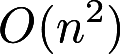
\includegraphics[width=0.43750in,height=0.19792in]{texmath/ead2f65Cdpi7B3507DO28n5E229},B正确,C选择排序即最简单的选出一个最大(最小)数据的排序方式,并非快速排序。D堆排序需要的额外存储空间为O(1),是最小的情况
\end{solution}
\question (中国科学院,2007年)若要求在O(nlogn)的时间内完成对数组的排序,且要求是稳定的,则可选择的排序方法是(
)
\par\twoch{快速排序}{堆排序}{\textcolor{red}{归并排序}}{直接插入排序}
\begin{solution}快速排序和堆排序不稳定,直接插入排序的时间复杂度是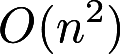
\includegraphics[width=0.43750in,height=0.19792in]{texmath/ead2f65Cdpi7B3507DO28n5E229}
\end{solution}
\question 排序趟数与序列的原始状态无关的排序方法是( )。 Ⅰ.直接插入排序
Ⅱ.简单选择排序 Ⅲ.冒泡排序 Ⅳ.基数排序
\par\twoch{仅Ⅰ、Ⅲ}{\textcolor{red}{仅Ⅰ、Ⅱ、Ⅳ}}{仅Ⅰ、Ⅱ、Ⅲ}{仅Ⅰ、Ⅳ}
\begin{solution}直接插入排序:每趟排序都是插入一个元素,所以排序趟数固定为n-1(n为元素数)。
简单选择排序:每趟排序都是选出一个最小(或最大)的元素,所以排序趟数固定为n-1(n为元素数)。
交换类的排序:其趟数和原始序列状态有关,所以冒泡排序与初始序列有关。
基数排序:每趟排序都要进行``分配''和``收集'',排序趟数固定为d(d为组成元素的关键字位数)。
综上所述,Ⅰ、Ⅱ、Ⅳ都是无关的,所以选B。
\end{solution}
